

\tikzset{every picture/.style={line width=0.75pt}} %set default line width to 0.75pt        

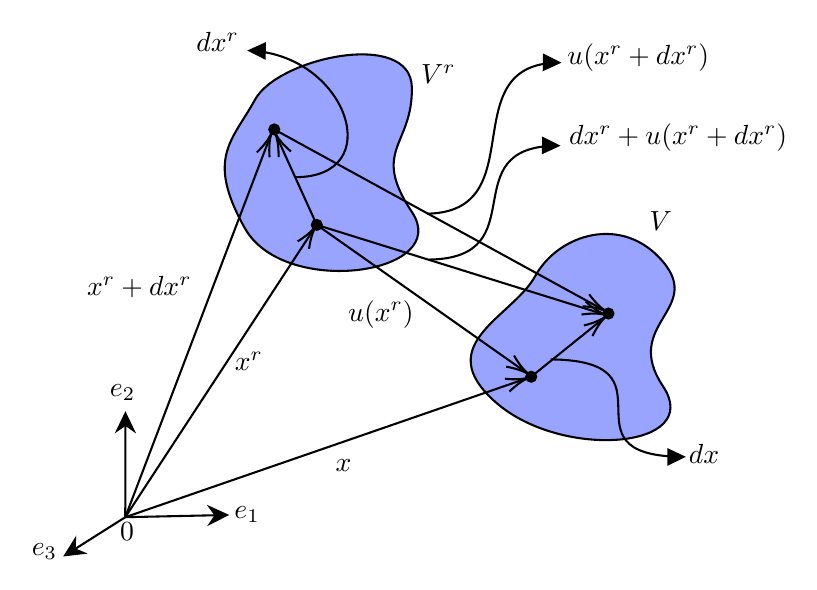
\begin{tikzpicture}[x=0.75pt,y=0.75pt,yscale=-1,xscale=1]
%uncomment if require: \path (0,292); %set diagram left start at 0, and has height of 292

%Shape: Polygon Curved [id:ds08619916045221121] 
\draw  [fill={rgb, 255:red, 0; green, 27; blue, 255 }  ,fill opacity=0.4 ] (427.5,132.8) .. controls (438.5,112.8) and (469.5,102.8) .. (489,126) .. controls (508.5,149.2) and (469,156) .. (489,186) .. controls (509,216) and (440.5,221.8) .. (408.5,193.8) .. controls (376.5,165.8) and (416.5,152.8) .. (427.5,132.8) -- cycle ;
%Shape: Polygon Curved [id:ds680978509087605] 
\draw  [fill={rgb, 255:red, 0; green, 27; blue, 255 }  ,fill opacity=0.4 ] (292.5,47.8) .. controls (303.5,27.8) and (367.5,13.8) .. (368,42) .. controls (368.5,70.2) and (348,72) .. (368,102) .. controls (388,132) and (306.5,143.8) .. (287.5,109.8) .. controls (268.5,75.8) and (281.5,67.8) .. (292.5,47.8) -- cycle ;
%Straight Lines [id:da27775957706905996] 
\draw    (322.2,108.25) -- (422.62,179.02) ;
\draw [shift={(424.26,180.17)}, rotate = 215.17000000000002] [color={rgb, 255:red, 0; green, 0; blue, 0 }  ][line width=0.75]    (10.93,-3.29) .. controls (6.95,-1.4) and (3.31,-0.3) .. (0,0) .. controls (3.31,0.3) and (6.95,1.4) .. (10.93,3.29)   ;
%Straight Lines [id:da02940601389234554] 
\draw    (322.2,108.25) -- (459.26,150.95) ;
\draw [shift={(461.17,151.54)}, rotate = 197.3] [color={rgb, 255:red, 0; green, 0; blue, 0 }  ][line width=0.75]    (10.93,-3.29) .. controls (6.95,-1.4) and (3.31,-0.3) .. (0,0) .. controls (3.31,0.3) and (6.95,1.4) .. (10.93,3.29)   ;
%Straight Lines [id:da04858175368526485] 
\draw    (229.92,249.08) -- (320.59,110.53) ;
\draw [shift={(321.69,108.86)}, rotate = 483.2] [color={rgb, 255:red, 0; green, 0; blue, 0 }  ][line width=0.75]    (10.93,-3.29) .. controls (6.95,-1.4) and (3.31,-0.3) .. (0,0) .. controls (3.31,0.3) and (6.95,1.4) .. (10.93,3.29)   ;
%Straight Lines [id:da3572803601625445] 
\draw    (229.92,249.08) -- (422.37,182.54) ;
\draw [shift={(424.26,181.89)}, rotate = 520.9300000000001] [color={rgb, 255:red, 0; green, 0; blue, 0 }  ][line width=0.75]    (10.93,-3.29) .. controls (6.95,-1.4) and (3.31,-0.3) .. (0,0) .. controls (3.31,0.3) and (6.95,1.4) .. (10.93,3.29)   ;
%Shape: Circle [id:dp7963034541993572] 
\draw  [fill={rgb, 255:red, 0; green, 0; blue, 0 }  ,fill opacity=1 ] (319.8,108.25) .. controls (319.8,106.92) and (320.87,105.85) .. (322.2,105.85) .. controls (323.53,105.85) and (324.6,106.92) .. (324.6,108.25) .. controls (324.6,109.58) and (323.53,110.65) .. (322.2,110.65) .. controls (320.87,110.65) and (319.8,109.58) .. (319.8,108.25) -- cycle ;
%Shape: Circle [id:dp5549951934814357] 
\draw  [fill={rgb, 255:red, 0; green, 0; blue, 0 }  ,fill opacity=1 ] (423.1,181.4) .. controls (423.1,180.07) and (424.17,179) .. (425.5,179) .. controls (426.83,179) and (427.9,180.07) .. (427.9,181.4) .. controls (427.9,182.73) and (426.83,183.8) .. (425.5,183.8) .. controls (424.17,183.8) and (423.1,182.73) .. (423.1,181.4) -- cycle ;
%Straight Lines [id:da09097339056268305] 
\draw    (229.92,249.08) -- (230,201) ;
\draw [shift={(230,198)}, rotate = 450.09] [fill={rgb, 255:red, 0; green, 0; blue, 0 }  ][line width=0.08]  [draw opacity=0] (10.72,-5.15) -- (0,0) -- (10.72,5.15) -- (7.12,0) -- cycle    ;
%Straight Lines [id:da3893826545167065] 
\draw    (229.92,249.08) -- (277,248.06) ;
\draw [shift={(280,248)}, rotate = 538.76] [fill={rgb, 255:red, 0; green, 0; blue, 0 }  ][line width=0.08]  [draw opacity=0] (10.72,-5.15) -- (0,0) -- (10.72,5.15) -- (7.12,0) -- cycle    ;
%Straight Lines [id:da21469655729558346] 
\draw    (229.92,249.08) -- (202.54,266.4) ;
\draw [shift={(200,268)}, rotate = 327.69] [fill={rgb, 255:red, 0; green, 0; blue, 0 }  ][line width=0.08]  [draw opacity=0] (10.72,-5.15) -- (0,0) -- (10.72,5.15) -- (7.12,0) -- cycle    ;
%Straight Lines [id:da4866033538311314] 
\draw    (425.5,181.4) -- (459.9,153.66) ;
\draw [shift={(461.46,152.4)}, rotate = 501.11] [color={rgb, 255:red, 0; green, 0; blue, 0 }  ][line width=0.75]    (10.93,-3.29) .. controls (6.95,-1.4) and (3.31,-0.3) .. (0,0) .. controls (3.31,0.3) and (6.95,1.4) .. (10.93,3.29)   ;
%Curve Lines [id:da9181705698289111] 
\draw    (434.9,173.05) .. controls (497.94,173.71) and (437.92,218.91) .. (497.21,219.98) ;
\draw [shift={(500,220)}, rotate = 539.73] [fill={rgb, 255:red, 0; green, 0; blue, 0 }  ][line width=0.08]  [draw opacity=0] (8.93,-4.29) -- (0,0) -- (8.93,4.29) -- cycle    ;
%Straight Lines [id:da8085286493536537] 
\draw    (322.2,108.25) -- (303.08,66.11) ;
\draw [shift={(302.26,64.29)}, rotate = 425.6] [color={rgb, 255:red, 0; green, 0; blue, 0 }  ][line width=0.75]    (10.93,-3.29) .. controls (6.95,-1.4) and (3.31,-0.3) .. (0,0) .. controls (3.31,0.3) and (6.95,1.4) .. (10.93,3.29)   ;
%Straight Lines [id:da06391364265309418] 
\draw    (301.7,62.25) -- (459.7,148.87) ;
\draw [shift={(461.46,149.83)}, rotate = 208.73] [color={rgb, 255:red, 0; green, 0; blue, 0 }  ][line width=0.75]    (10.93,-3.29) .. controls (6.95,-1.4) and (3.31,-0.3) .. (0,0) .. controls (3.31,0.3) and (6.95,1.4) .. (10.93,3.29)   ;
%Curve Lines [id:da6195997993819029] 
\draw [color={rgb, 255:red, 0; green, 0; blue, 0 }  ,draw opacity=1 ]   (311.95,85.25) .. controls (356.05,85.25) and (337.48,27.63) .. (291.55,24.38) ;
\draw [shift={(288.7,24.25)}, rotate = 361.19] [fill={rgb, 255:red, 0; green, 0; blue, 0 }  ,fill opacity=1 ][line width=0.08]  [draw opacity=0] (8.93,-4.29) -- (0,0) -- (8.93,4.29) -- cycle    ;
%Curve Lines [id:da8347033822514986] 
\draw    (375.2,102.85) .. controls (427.05,102.09) and (387.51,31.48) .. (437.68,30.09) ;
\draw [shift={(440.04,30.08)}, rotate = 180.82] [fill={rgb, 255:red, 0; green, 0; blue, 0 }  ][line width=0.08]  [draw opacity=0] (8.93,-4.29) -- (0,0) -- (8.93,4.29) -- cycle    ;
%Curve Lines [id:da7704708098624058] 
\draw    (376.36,124.96) .. controls (428.21,124.2) and (387.15,70.95) .. (437.29,70.08) ;
\draw [shift={(439.64,70.08)}, rotate = 180.82] [fill={rgb, 255:red, 0; green, 0; blue, 0 }  ][line width=0.08]  [draw opacity=0] (8.93,-4.29) -- (0,0) -- (8.93,4.29) -- cycle    ;
%Straight Lines [id:da08511227281768252] 
\draw    (229.92,249.08) -- (299.55,66.15) ;
\draw [shift={(300.26,64.29)}, rotate = 470.84] [color={rgb, 255:red, 0; green, 0; blue, 0 }  ][line width=0.75]    (10.93,-3.29) .. controls (6.95,-1.4) and (3.31,-0.3) .. (0,0) .. controls (3.31,0.3) and (6.95,1.4) .. (10.93,3.29)   ;
%Shape: Circle [id:dp47512159867268555] 
\draw  [fill={rgb, 255:red, 0; green, 0; blue, 0 }  ,fill opacity=1 ] (299.3,62.25) .. controls (299.3,60.92) and (300.37,59.85) .. (301.7,59.85) .. controls (303.03,59.85) and (304.1,60.92) .. (304.1,62.25) .. controls (304.1,63.58) and (303.03,64.65) .. (301.7,64.65) .. controls (300.37,64.65) and (299.3,63.58) .. (299.3,62.25) -- cycle ;
%Shape: Circle [id:dp20685874584691932] 
\draw  [fill={rgb, 255:red, 0; green, 0; blue, 0 }  ,fill opacity=1 ] (460.3,150.95) .. controls (460.3,149.62) and (461.37,148.55) .. (462.7,148.55) .. controls (464.03,148.55) and (465.1,149.62) .. (465.1,150.95) .. controls (465.1,152.28) and (464.03,153.35) .. (462.7,153.35) .. controls (461.37,153.35) and (460.3,152.28) .. (460.3,150.95) -- cycle ;

% Text Node
\draw (281,242.4) node [anchor=north west][inner sep=0.75pt]    {$\vt{e}_{1}$};
% Text Node
\draw (329.71,219.64) node [anchor=north west][inner sep=0.75pt]    {$\vt{x}$};
% Text Node
\draw (281.21,168.04) node [anchor=north west][inner sep=0.75pt]    {$\vt{x}^{r}$};
% Text Node
\draw (371,29.4) node [anchor=north west][inner sep=0.75pt]    {$V^{r}$};
% Text Node
\draw (481,100.4) node [anchor=north west][inner sep=0.75pt]    {$V$};
% Text Node
\draw (221,183.6) node [anchor=north west][inner sep=0.75pt]    {$\vt{e}_{2}$};
% Text Node
\draw (183.4,260.2) node [anchor=north west][inner sep=0.75pt]    {$\vt{e}_{3}$};
% Text Node
\draw (335.83,143.07) node [anchor=north west][inner sep=0.75pt]    {$\vt{u}(\vt{x}^r)$};
% Text Node
\draw (226,250.4) node [anchor=north west][inner sep=0.75pt]    {$0$};
% Text Node
\draw (500,212.4) node [anchor=north west][inner sep=0.75pt]    {$d\vt{x}$};
% Text Node
\draw (262.67,13.73) node [anchor=north west][inner sep=0.75pt]    {$d\vt{x}^{r}$};
% Text Node
\draw (441.47,19.53) node [anchor=north west][inner sep=0.75pt]    {$\vt{u}(\vt{x}^{r} +d\vt{x}^{r})$};
% Text Node
\draw (442.27,57.93) node [anchor=north west][inner sep=0.75pt]    {$d\vt{x}^{r}+\vt{u}(\vt{x}^{r} +d\vt{x}^{r})$};
% Text Node
\draw (210.07,131.53) node [anchor=north west][inner sep=0.75pt]    {$\vt{x}^{r} +d\vt{x}^{r}$};

\end{tikzpicture}
